% !TEX root = ../../main_without_quantization.tex
% Required in the preamble:
% \usepackage{graphicx}
% \usepackage{float}
% \usepackage{array}

\section{Technical Architecture of the Solution}

The proposed solution follows a modular technical architecture: load a pretrained Transformer, prepare the task data, define the baseline fine-tuning setup, search for a compressed architecture, recover the selected candidate when required, and evaluate the final model. The implementation pattern is shared across compression families; only the candidate representation and budget measure change.

The search operates on the active compression family: structural masks for encoder pruning, kept or skipped sub-blocks for layer dropping, bit-width levels for quantization, and rank levels for low-rank methods. After selection, optional recovery fine-tuning adapts the chosen candidate, then evaluation saves the final checkpoints, metrics, logs, and figures. Figure~\ref{fig:technical_architecture_pipeline} summarizes this end-to-end architecture.

\begin{figure}[H]

\makebox[\textwidth][l]{%
\hspace*{-0.15\textwidth}%
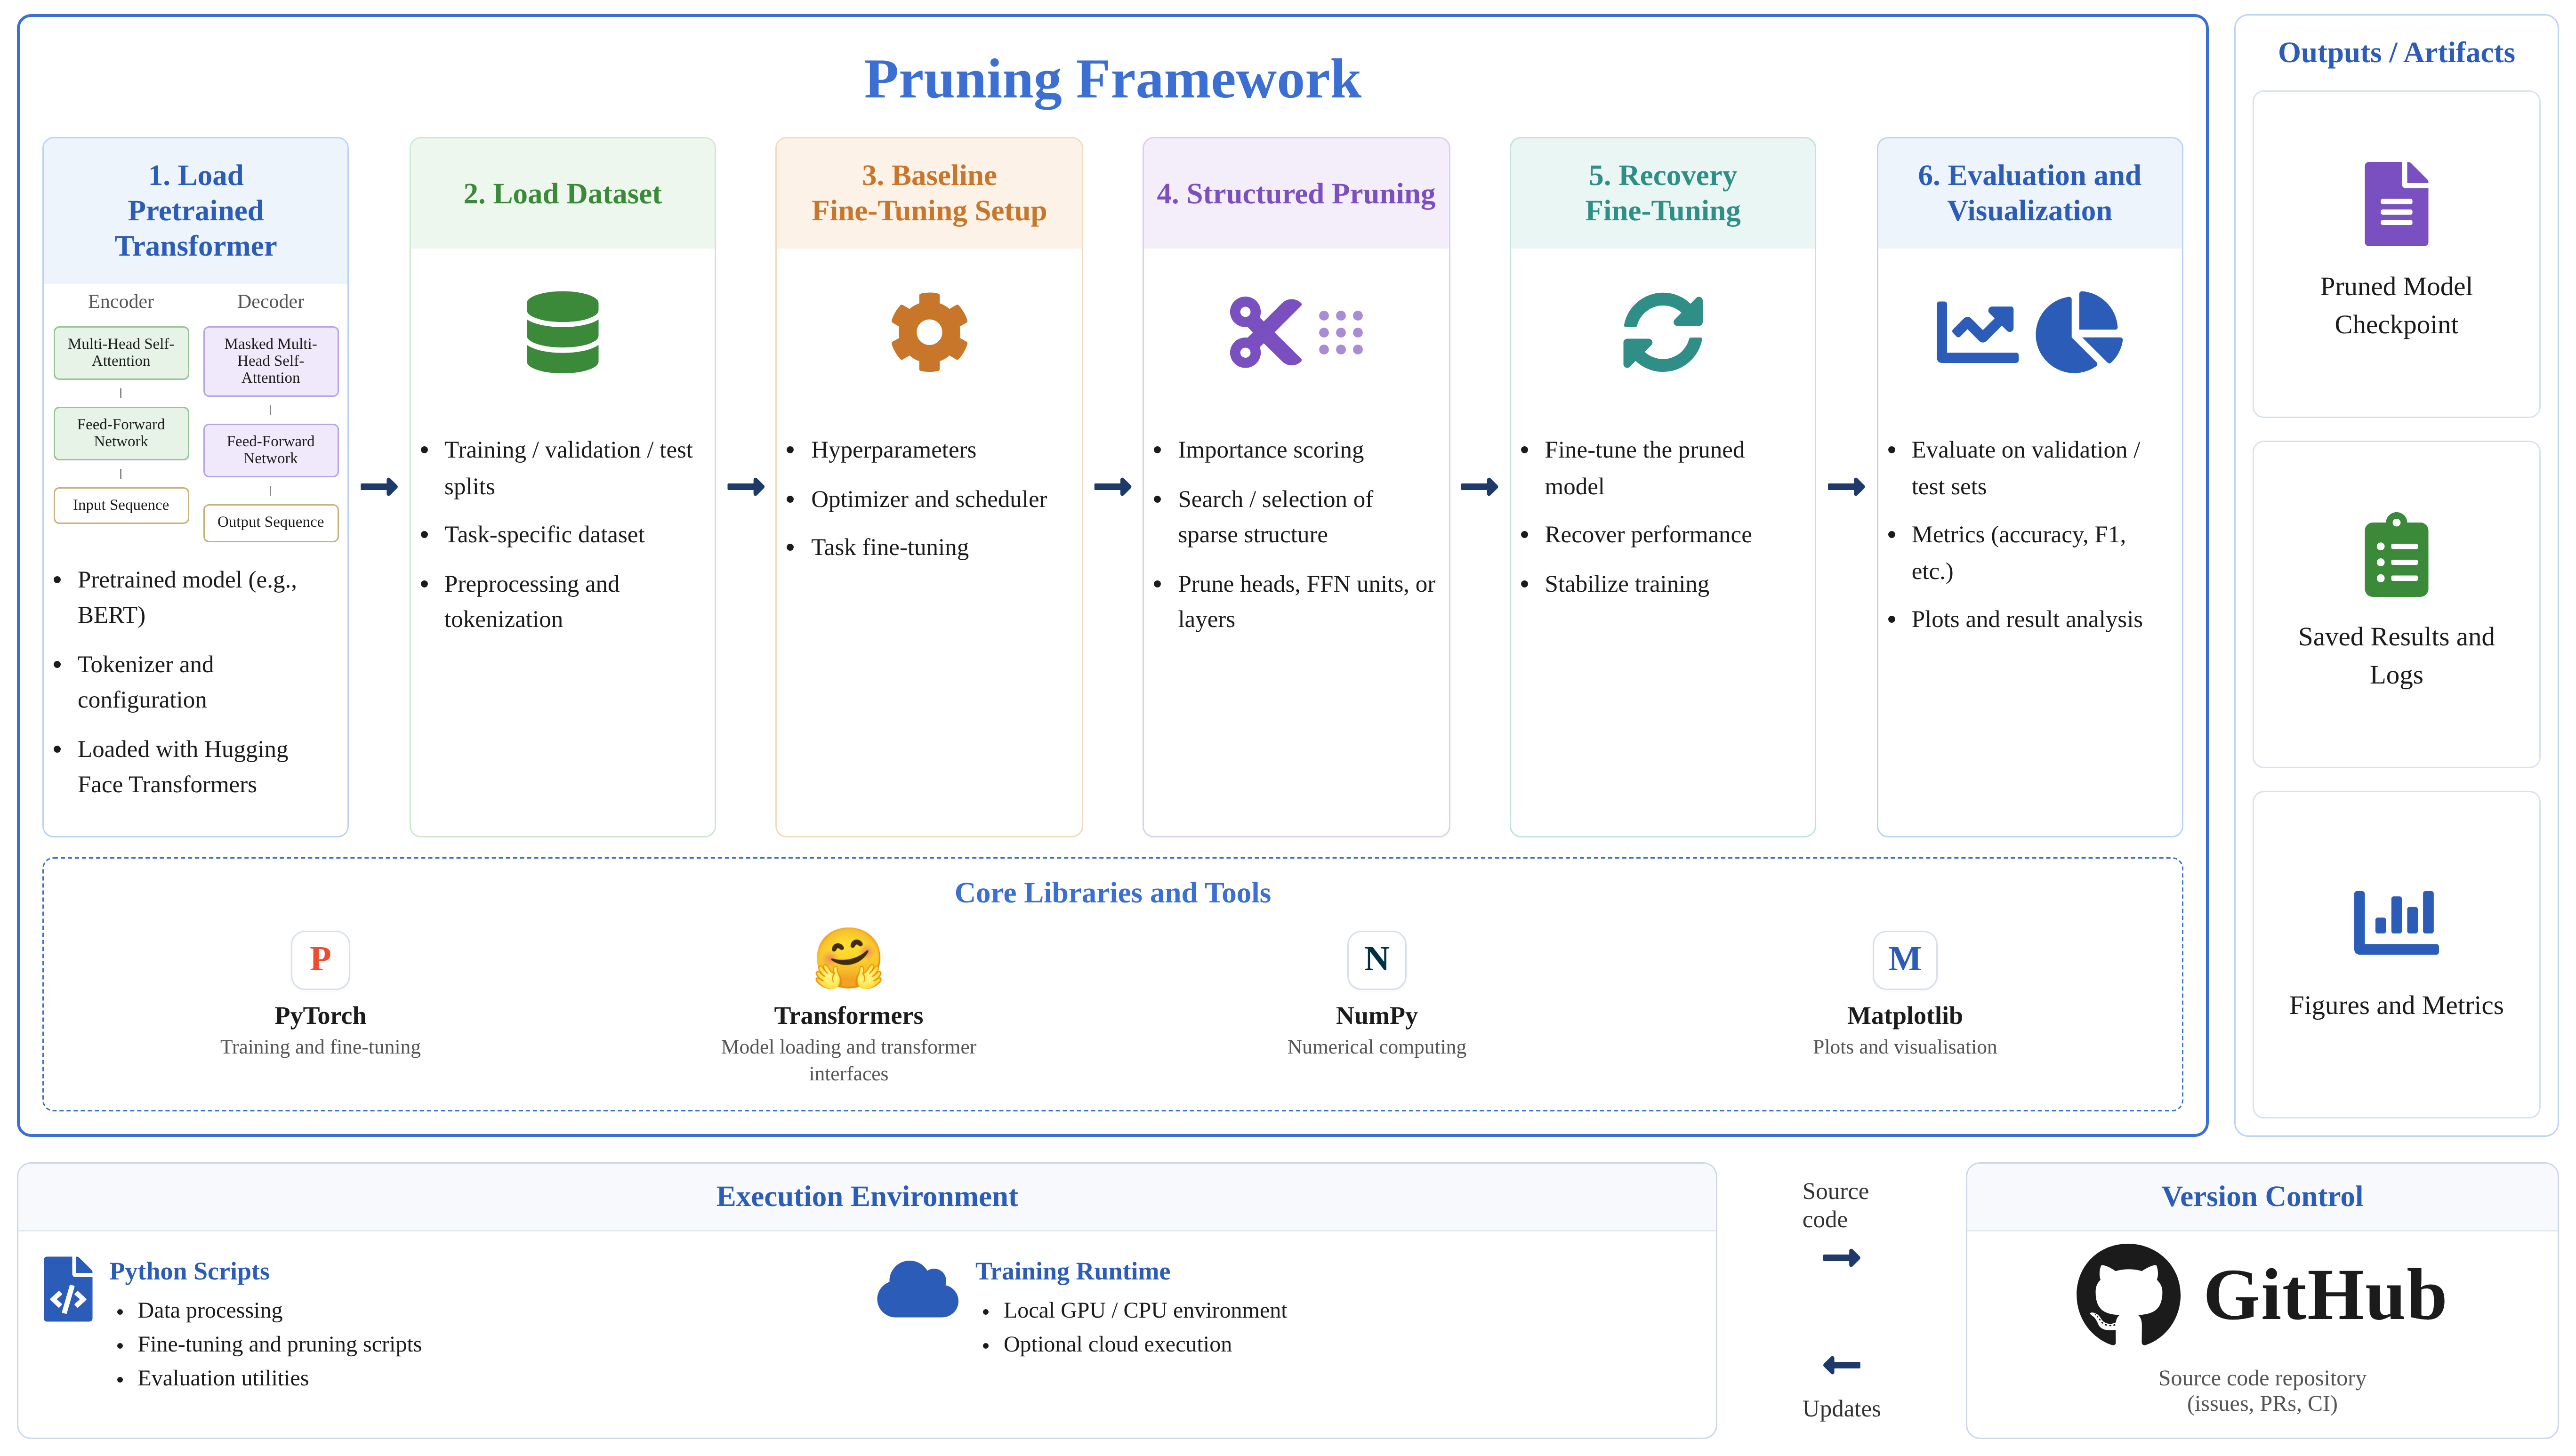
\includegraphics[width=1.3\textwidth,height=0.7\textheight,keepaspectratio]{pipeline.png}%
}
\caption{Technical pipeline of the implemented compression framework. A pretrained Transformer and task dataset are loaded first, a baseline setup fixes the training configuration, the search stage selects a compressed architecture under the active budget constraint, recovery fine-tuning adapts the selected candidate when needed, and the final stage evaluates the model and saves checkpoints, metrics, logs, and figures.}
\label{fig:technical_architecture_pipeline}
\end{figure}

\section{Technologies Used}

This section presents the main technologies used during the design, implementation, experimentation, and management of the proposed solution. These tools provide the required environment for deep learning development, numerical computation, visualization, experiment execution, version control, and project organization.

\subsection{Python}

Python is an open-source, high-level programming language widely used in software development, scientific computing, data analysis, and artificial intelligence. Its ecosystem provides libraries for model implementation, numerical processing, data handling, and experiment automation. The pruning pipeline, training scripts, evaluation scripts, search procedures, and experiment utilities were implemented in Python \cite{pythonAbout,pythonDocs}.

\begin{figure}[H]
	\centering
	
\includegraphics[width=0.35\textwidth]{figures/psf.png}
	\caption{Python logo.}
	\label{fig:python-logo}
\end{figure}

\subsection{Transformers}

Transformers is an open-source library developed by Hugging Face. It provides a unified interface for loading pretrained Transformer models, tokenizers, configuration files, and task-specific model heads \cite{wolf2020transformers,huggingfaceTransformersDocs}.

The implementation uses this library to load the pretrained encoder model and access its internal components. These components include encoder layers, attention modules, feed-forward submodules, hidden states, attention outputs, configuration parameters, and classification heads. Structured pruning requires access to these components because the method removes complete computational units from the model.

Pruning an attention head requires identifying the corresponding projection dimensions inside the attention module. Pruning feed-forward neurons requires selecting intermediate dimensions inside the two-layer feed-forward network. The Transformers library provides a standardized model structure that supports these operations without requiring a complete reimplementation of the architecture.

\begin{figure}[H]
	\centering
	
\includegraphics[width=0.38\textwidth]{figures/transformers.png}
	\caption{Hugging Face Transformers logo.}
	\label{fig:transformers-logo}
\end{figure}

\subsection{PyTorch}

PyTorch is an open-source deep learning framework that provides tensor computation, automatic differentiation, and GPU acceleration. It is commonly used for building, training, and evaluating neural networks. The implementation relies on PyTorch to execute forward passes, compute losses, perform backpropagation, apply masks, update model weights, and run recovery fine-tuning \cite{pytorchDocs,pytorchProject}.

PyTorch is also used to represent pruning masks as tensors. An attention-head mask can be represented as a binary tensor of shape $12 \times 12$ for a model with twelve layers and twelve heads per layer. A feed-forward mask can be represented as a binary tensor of shape $12 \times 3072$ for twelve layers and $3072$ intermediate neurons per layer.

\begin{figure}[H]
	\centering
	
\includegraphics[width=0.35\textwidth]{figures/pytorch.png}
	\caption{PyTorch logo.}
	\label{fig:pytorch-logo}
\end{figure}

\subsection{NumPy}

NumPy is a fundamental Python library for numerical and scientific computing. It provides efficient multidimensional arrays, mathematical operations, random number generation, and linear algebra utilities. NumPy is used for candidate representation, statistical calculations, random sampling, sorting operations, and search-related utilities \cite{numpyOfficial,numpyPyPI}.

Candidate architectures can be stored as arrays indicating the number of active heads and neurons per layer. These arrays are then used to calculate sparsity, compare candidates, and enforce computational constraints.

\begin{figure}[H]
	\centering
	
\includegraphics[width=0.35\textwidth]{figures/numpy_logo.png}
	\caption{NumPy logo.}
	\label{fig:numpy-logo}
\end{figure}

\subsection{Matplotlib}

Matplotlib is a Python library used to create static, animated, and interactive visualizations. It is used to present experimental results, search behavior, pruning statistics, training curves, and comparisons between candidate architectures \cite{matplotlibDocs,matplotlibOfficial}.

Typical visualizations include validation accuracy after recovery, active heads per layer, preserved feed-forward neurons per layer, and the relationship between computational cost and task performance.

\begin{figure}[H]
	\centering
	
\includegraphics[width=0.38\textwidth]{figures/matplotlib.png}
	\caption{Matplotlib logo.}
	\label{fig:matplotlib-logo}
\end{figure}

\subsection{Google Drive}

Google Drive is a cloud storage service that allows files to be uploaded, stored, shared, and accessed from different devices. It is used to organize project files, store experimental outputs, keep backup copies of important resources, and transfer files between working environments \cite{googleDriveOfficial}.

\begin{figure}[H]
	\centering
	
\includegraphics[width=0.34\textwidth]{figures/gd.png}
	\caption{Google Drive logo.}
	\label{fig:google-drive-logo}
\end{figure}

\subsection{Git}

Git is a free and open-source distributed version control system designed to track changes in source code and support collaborative software development. It is used to track modifications to the implementation, preserve experiment scripts, compare previous versions, and maintain a structured development history \cite{gitOfficial,gitBook}.

\begin{figure}[H]
	\centering
	
\includegraphics[width=0.34\textwidth]{figures/git.png}
	\caption{Git logo.}
	\label{fig:git-logo}
\end{figure}

\subsection{GitHub}

GitHub is a cloud-based platform built around Git. It allows developers to store, manage, share, and collaborate on code through repositories. It is used to host the project repository, synchronize code between machines, and maintain a remote copy of the implementation \cite{githubDocs,githubOfficial}.

\begin{figure}[H]
	\centering
	
\includegraphics[width=0.34\textwidth]{figures/github.png}
	\caption{GitHub logo.}
	\label{fig:github-logo}
\end{figure}

\section{Datasets Used}
\label{sec:datasets}

The experimental evaluation uses supervised natural language understanding tasks. These tasks evaluate sentence classification and sentence-pair reasoning after structured pruning.

The selected benchmarks are SST-2, QNLI, and MNLI from the GLUE benchmark \citep{wang2018glue}. The dataset discussion is limited to the required information because the main focus of the project is structured model pruning.

\subsection{Pre-Training Corpora}
\label{subsec:pretraining-corpora}

The pretrained encoder model was originally trained on BooksCorpus and English Wikipedia \citep{devlin2019bert,zhu2015aligning}. BooksCorpus provides long narrative text from unpublished books. English Wikipedia provides factual and encyclopaedic text. These corpora provide broad linguistic representations before supervised task adaptation.

The model uses WordPiece tokenisation \citep{wu2016googles}. Frequent words are represented as complete tokens, while rare words are decomposed into subword units. For example, a rare morphological form can be split into smaller units instead of being mapped to an unknown token. The same tokenizer is preserved during fine-tuning, pruning, and evaluation.

\subsection{Fine-Tuning and Evaluation Benchmarks}
\label{subsec:finetuning-evaluation-benchmarks}

Table~\ref{tab:dataset-examples} presents the selected evaluation tasks, including their input format, label space, and representative labelled examples.

\begin{table}[H]
	\centering
	\scriptsize
	\setlength{\tabcolsep}{3pt}
	\begin{tabularx}{\textwidth}{|>{\raggedright\arraybackslash}p{0.12\textwidth}|X|>{\raggedright\arraybackslash}p{0.24\textwidth}|>{\raggedright\arraybackslash}p{0.16\textwidth}|}
		\hline
		\textbf{Task} & \textbf{Example Input} & \textbf{Possible Labels} & \textbf{Correct Label} \\
		\hline
		SST-2 &
		Sentence: \textit{``The movie is beautifully acted and emotionally powerful.''} &
		\texttt{positive}, \texttt{negative} &
		\texttt{positive} \\
		\hline
		SST-2 &
		Sentence: \textit{``The story is dull, slow, and completely forgettable.''} &
		\texttt{positive}, \texttt{negative} &
		\texttt{negative} \\
		\hline
		QNLI &
		Question: \textit{``Where is the Eiffel Tower located?''}
		
		Sentence: \textit{``The Eiffel Tower is located in Paris, France.''} &
		\texttt{entailment}, \texttt{not\_entailment} &
		\texttt{entailment} \\
		\hline
		QNLI &
		Question: \textit{``Where is the Eiffel Tower located?''}
		
		Sentence: \textit{``The Eiffel Tower was completed in 1889.''} &
		\texttt{entailment}, \texttt{not\_entailment} &
		\texttt{not\_entailment} \\
		\hline
		MNLI &
		Premise: \textit{``A man is playing a guitar on stage.''}
		
		Hypothesis: \textit{``A person is performing music.''} &
		\texttt{entailment}, \texttt{contradiction}, \texttt{neutral} &
		\texttt{entailment} \\
		\hline
		MNLI &
		Premise: \textit{``A man is playing a guitar on stage.''}
		
		Hypothesis: \textit{``No one is playing an instrument.''} &
		\texttt{entailment}, \texttt{contradiction}, \texttt{neutral} &
		\texttt{contradiction} \\
		\hline
		MNLI &
		Premise: \textit{``A man is playing a guitar on stage.''}
		
		Hypothesis: \textit{``The man is performing in a crowded theatre.''} &
		\texttt{entailment}, \texttt{contradiction}, \texttt{neutral} &
		\texttt{neutral} \\
		\hline
	\end{tabularx}
	\caption{Input formats and label spaces for the selected evaluation tasks.}
	\label{tab:dataset-examples}
\end{table}

\subsubsection{SST-2}
\label{subsubsec:sst2}

SST-2 is a binary sentiment classification task derived from the Stanford Sentiment Treebank \citep{socher2013recursive}. Each input is a single sentence, and the model predicts whether its sentiment is \texttt{positive} or \texttt{negative}.

This task provides a sentence-level evaluation of the compressed model. A model must distinguish positive expressions such as \textit{``excellent and moving''} from negative expressions such as \textit{``boring and weak''}. Accuracy is used as the evaluation metric.

\subsubsection{QNLI}
\label{subsubsec:qnli}

QNLI is derived from the Stanford Question Answering Dataset \citep{rajpurkar2016squad}. It is formulated as a sentence-pair classification task. The input contains a question and a candidate sentence. The model predicts one of two labels: \texttt{entailment} or \texttt{not\_entailment}.

A label of \texttt{entailment} indicates that the sentence contains the answer to the question. A label of \texttt{not\_entailment} indicates that the sentence does not provide the requested information. For example, if the question asks where the Eiffel Tower is located, the sentence \textit{``The Eiffel Tower is located in Paris, France''} receives the label \texttt{entailment}. The sentence \textit{``The Eiffel Tower was completed in 1889''} receives the label \texttt{not\_entailment}.

This task evaluates the ability of the compressed model to compare two text segments. Accuracy is used as the evaluation metric.

\subsubsection{MNLI}
\label{subsubsec:mnli}

MNLI is a natural language inference task \citep{williams2018broad}. Each input contains a premise and a hypothesis. The model predicts one of three labels: \texttt{entailment}, \texttt{contradiction}, or \texttt{neutral}.

A label of \texttt{entailment} indicates that the hypothesis follows from the premise. A label of \texttt{contradiction} indicates that the hypothesis is incompatible with the premise. A label of \texttt{neutral} indicates that the hypothesis may be possible without being guaranteed by the premise.

For example, given the premise \textit{``A man is playing a guitar on stage''}, the hypothesis \textit{``A person is performing music''} receives the label \texttt{entailment}. The hypothesis \textit{``No one is playing an instrument''} receives the label \texttt{contradiction}. The hypothesis \textit{``The man is performing in a crowded theatre''} receives the label \texttt{neutral}, since the premise does not specify the audience or the exact venue.

MNLI provides a stronger sentence-pair reasoning evaluation than single-sentence sentiment classification. Accuracy is used as the reported metric.

\subsection{Language Model Evaluation Datasets}
\label{subsec:lm-datasets}

The language model pruning experiments use three standard perplexity benchmarks to evaluate the compressed models.

\subsubsection{WikiText-2}
WikiText-2 is a word-level language modelling benchmark derived from verified Good and Featured Wikipedia articles \citep{merity2017pointer}. It provides a clean, coherent corpus of encyclopaedic text. Perplexity on the test split is the standard evaluation metric; lower values indicate better language modelling quality.

\subsubsection{C4}
C4 (Colossal Clean Crawled Corpus) is a large-scale web text corpus produced by applying aggressive filtering and deduplication to Common Crawl snapshots \citep{raffel2020exploring}. It covers a broad range of domains and writing styles and is commonly used both as a pretraining source and as an out-of-domain perplexity benchmark for evaluating generalisation after compression.

\subsubsection{FineWeb-Edu}
FineWeb-Edu is a high-quality subset of the FineWeb web corpus filtered for educational content \citep{lozhkov2024fineweb_edu}. The filtering pipeline uses a classifier trained to identify instructional and informative text. It provides a more domain-specific evaluation signal than general web corpora and has been adopted as a benchmark for assessing language model quality on structured, factual text.

\section{Model}
\label{sec:models}

\subsection{BERT}
\label{subsec:bert}

BERT is an encoder-only Transformer architecture trained with masked language modelling and next-sentence prediction \citep{devlin2019bert,vaswani2017attention}. Its bidirectional self-attention allows each token representation to incorporate information from both left and right context.

BERT\textsubscript{BASE} contains twelve Transformer encoder layers. Each layer has twelve attention heads and a feed-forward block with intermediate width $3072$. The hidden size is $768$, and the full model contains approximately $110$ million parameters. For classification tasks, the representation of the \texttt{[CLS]} token is passed to a task-specific classifier.

The pruning procedure targets structured units inside the encoder blocks. Attention heads and feed-forward neurons are removed as complete units. This pruning form supports practical acceleration because it can reduce matrix dimensions and remove complete computational paths.

For example, if layer $3$ preserves only $2$ attention heads out of $12$, then the attention computation in that layer is reduced. If the same layer preserves only $192$ feed-forward neurons out of $3072$, then the intermediate feed-forward projection is also reduced. The final compressed architecture is therefore described by its total sparsity and by the distribution of preserved units across layers.

\subsection{EleutherAI Pythia-1.4B}
\label{subsec:pythia}

Pythia is a suite of autoregressive decoder-only language models released by EleutherAI and trained on The Pile, a diverse 825\,GB English text corpus \citep{biderman2023pythia}. The suite spans eight model sizes from 70M to 12B parameters and was designed to support reproducible research on scaling laws, training dynamics, and model analysis.

Pythia-1.4B contains 24 Transformer decoder layers with a hidden dimension of 2048, 16 attention heads per layer, and a feed-forward intermediate width of 8192. The model has approximately 1.4 billion parameters. It uses rotary position embeddings and parallel attention and feed-forward computation within each layer.

This model is selected for the language model pruning experiments because its size is tractable for iterative search-based compression on a single GPU, while being large enough to exhibit realistic structured redundancy across layers. Perplexity on WikiText-2, C4, and FineWeb-Edu is used as the evaluation metric.

\section{Experimental Environment}
\label{sec:experimental-environment}

All experiments are conducted on a laptop equipped with an NVIDIA RTX 4090 Laptop GPU with 16\,GB of VRAM. Model loading, tokenization, fine-tuning, pruning, checkpoint handling, and evaluation are implemented using the Hugging Face Transformers library \citep{wolf2020transformers}.

Mixed precision training is used when numerically stable \citep{micikevicius2018mixed}. It reduces memory consumption and can improve throughput on compatible hardware. Numerical stability is monitored during recovery fine-tuning, especially for highly compressed architectures.

The hardware environment imposes practical constraints on the experimental protocol. Laptop GPUs are affected by thermal limits, power configuration, driver behavior, and cooling conditions. Therefore, wall-clock measurements are hardware-dependent. Small accuracy differences are interpreted cautiously because repeated runs may vary due to random initialization, data ordering, dropout, and GPU-level nondeterminism.

\subsection{Baselines and Reporting}

Included in the comparison is our search approach and random, beam search and structured pruning comparisons, drawing structured pruning refs from CoFi \citep{xia2022cofi} and ZipLM \citep{kurtic2023ziplm}. Comparisons are made at the same constraints where possible, particularly the target computation budget, recovery process and measure.

For the decoder-model searches on Pythia-1.4B (layer drop, quant and low-rank factorisation), we compare against EvoPress \citep{evopress2024}, a search-based approach whose evolutionary algorithm and KL-divergence fitness are most similar to our approach. Both methods are run at the same sparsity or bit-width target and compared over the same perplexity datasets.

\subsection{Level Database and Token Budgets}

Both the quantization and the low-rank search are performed on a level database that has been generated beforehand. For each weight matrix, weights are pre-compressed to every possible level and persisted to disk: one GPTQ-quantized copy at each bit-width, and a truncated-SVD factor pair at each rank (plus the residue singular triplets required to recover weights). During search, each candidate is assembled by loading the required weights whose names are specified by its per-layer level vector. No decompression or on-the-fly compression happens and each query takes one forward pass.

Each of the searches tunes to approximately 250,000 held-out tokens. This is well below the budgets spent by the bigger baseline models, and necessary given the 16 GB of VRAM on the GPU. Candidates are scored using the multi-stage process described in Section~\ref{chap:ga} above: the early stages screen the population efficiently by spending a limited number of tokens per candidate, and the remaining candidates are then scored on more tokens to make the selection. Final perplexity is reported over the entire test sets.